\section{Hydrostatik}

\subsection{Festkörper, Flüssigkeit, Gas}

\subsubsection{Festkörper}

\begin{tabular}{ll}
	$\bullet$ & kein Fluid \\
	$\bullet$ & festes Volumen; feste Gestalt \\
	$\bullet$ & Moleküle / Atome befinden sich in regelmässiger \\
			  & Gitter-Anordnung \\
	$\bullet$ & inkompressibel (sehr schlecht komprimierbar) \\
	$\bullet$ & Kraft: Weiterleitung (längs ihrer Wirkungslinie) \\
	$\bullet$ & Druck: Verstärkung \\
\end{tabular}

\subsubsection{ideale Flüssigkeit}

\begin{tabular}{ll}
	$\bullet$ & Fluid \\
	$\bullet$ & festes Volumen; keine feste Gestalt \\
	$\bullet$ & Moleküle / Atome bewegen sich chaotisch aneinander vorbei \\
	$\bullet$ & Moleküle / Atome füllen den Raum aus / berühren sich \\
	$\bullet$ & inkompressibel (schlecht komprimierbar) \\
	$\bullet$ & reibungsfrei (keine Scherkräfte)\\
	$\bullet$ & Kraft: Verstärkung \\
	$\bullet$ & Druck: Weiterleitung (gleichmässig) \\
\end{tabular}



\subsubsection{Gas}

\begin{tabular}{ll}
	$\bullet$ & Fluid \\
	$\bullet$ & kein festes Volumen; keine feste Gestalt \\
	$\bullet$ & Moleküle / Atome fliegen mit hoher Geschwindigkeit durch\\
			  & den Raum \\
	$\bullet$ & Es gibt sehr viel Zwischenraum \\
	$\bullet$ &  Moleküle / Atome führen bei Zusammenstoss unter sich oder\\
			  & mit Gefässwand elestische Stösse aus \\
	$\bullet$ & kompressibel (gut komprimierbar)  \\
	$\bullet$ & reibungsfrei (keine Scherkräfte)\\

\end{tabular}


% \vfill\null
% \columnbreak


\subsection{Druck $p$ / Schubspannung $\tau$}
\textbf{Druck ist eine skalare Grösse (hat keine Richtung)} 


$$\boxed{ p = \frac{F_{\perp}}{A} } \qquad \boxed{ \tau = \frac{F_{\parallel}}{A} } $$

	\begin{tabular}{c l c}
		$p$ & Druck & $[p] = \mathrm{Pa = \frac{N}{m^2}}$ \\
		$\tau$ & Schubspannung (Scherkraft) & $[\tau] = \mathrm{N} $ \\
		$F_{\perp}$ & Kraft senkrecht zu A & $[F_{\perp}] = \mathrm{N}$ \\
		$F_{\parallel}$ & Kraft parallel zu A & $[F_{\parallel}] = \mathrm{N}$ \\
		$A$ & Fläche & $[A] = \mathrm{m^2}$ \\
		\\
	\end{tabular}
	
	\textbf{In abgeschlossenen, miteinander verbundenen Systemen herrscht ein Druck-Gleichgewicht!} 
	
	$$ \boxed{ p_1 = p_2  \qquad \Rightarrow \frac{F_1}{A_1} = \frac{F_2}{A_2} }$$
	
	
	
	\subsubsection{Weitere Einheiten von Druck}
	\textbf{1 bar = $10^5$ Pa} \qquad (Absulutdruck: Vergleich zu Vakuum)\\
	$ 1 \, \mathrm{hPa} = 100 \, \mathrm{Pa} = 1 \, \mathrm{mbar}$ \\
	$1 \, \mathrm{at} = 1 \, \mathrm{kp \cdot cm^{-2}} = 9.81 \cdot 10^4 \, \mathrm{Pa}$  \\
	$1 \, \mathrm{at"u} = 1 \, \mathrm{at}$ ("Uberdruck; Vergleich zu normalem Luftdruck) \\
	$1 \, \mathrm{Torr} = \frac{1}{760} \mathrm{at}$ (1mm-Hg-Säule) \\
	$1 \, \mathrm{psi} = 6894.76 \, \mathrm{Pa}$ (Britisch) \\


	
	


\subsection{Kompression}
	
	
	$$ \boxed{ \text{Flüssigkeiten:} \qquad \Delta p = \frac{1}{\kappa} \cdot - \frac{\Delta V}{V} = K \cdot - \frac{\Delta V}{V} } $$  
	
	$$ \boxed{  \text{Gase:} \qquad \Delta p = p(h) - p_0 = \frac{1}{\kappa_T} \cdot - \frac{\Delta V}{V} } $$ \\
	
	
	
	\begin{tabular}{c l c}
		$\Delta p$ & Druckerhöhung & $[\Delta p] = \mathrm{Pa = \frac{N}{m^2}}$ \\
		$\kappa$ & Kompressibilität (Flüssigkeit) & $[\kappa] = \mathrm{\frac{1}{Pa}}$ \\
		$K = \frac{1}{\kappa}$ & Kompressionsmodul & $[K] = \mathrm{Pa}$ \\
		$\kappa_T$ & Kompressibilität (Gas) & $[\kappa_T] = \mathrm{\frac{1}{Pa}}$ \\
		$- \frac{\Delta V}{V}$ & realtive Volumen-Abnahme & $[\frac{\Delta V}{V}] = 1$ 
	\end{tabular}
	
	
	
\subsection{Dichte $\rho$}

$$ \boxed{ \rho = \frac{m}{V} } \qquad \Leftrightarrow \qquad \boxed{ m = \rho \cdot V }$$	 


	\begin{tabular}{c l c}
		$\rho$ & Dichte & $[\rho] = \mathrm{\frac{kg}{m^3}}$ \\
		$m$ & Masse & $[m] = \mathrm{kg} $ \\
		$V$ & Volumen & $[V] = \mathrm{m^3}$ \\
	\end{tabular}
	
	
\subsubsection{Wichtige Dichten}	
	
	\begin{tabular}{l}
		$\rho_{Wasser} = 1000 \, \mathrm{\frac{kg}{m^3}}  $ \\
		$\rho_{Luft} = 1.2 \, \mathrm{\frac{kg}{m^3}}  $ \\
	\end{tabular}
	
	
	
% \vfill\null
% \columnbreak
	
\subsection{Boyle-Mariotte}	
\textbf{Das Gesetz von Boyle-Mariotte beschreibt die \\
Kompressibilität von Gasen.} \\
\textbf{$\Rightarrow$ Das Gesetz gilt nur bei konstanter Temperatur!} \\

$$ \boxed{ p_1 \cdot V_1 = p_2 \cdot V_2 = \, \const } \qquad  \Rightarrow  \boxed{ \frac{p_1}{p_2} = \frac{\rho_1}{\rho_2} }$$ 


	\begin{tabular}{c l c}
		\rule{0pt}{8pt}$\rho_x$ & Gas-Dichte & $[\rho_x] = \mathrm{\frac{kg}{m^3}}$ \\
		$p_x$ & Gas-Druck & $[p_x] = \mathrm{Pa} $ \\
		$V_x$ & Volumen & $[V_x] = \mathrm{m^3}$ \\
	\end{tabular}
	
	
	
\subsection{Hydrostatischer Druck (Schweredruck)}
\textbf{Fluid inkompressibel!} 

$$ \boxed{ p = \rho \cdot g \cdot h }$$	


	\begin{tabular}{c l c}
		\rule{0pt}{8pt}$\rho$ & Dichte der Flüssigkeit & $[\rho] = \mathrm{\frac{kg}{m^3}}$ \\
		\rule{0pt}{8pt}$g$ & Erdbeschleunigung $g = 9.81 \mathrm{\frac{m}{s^2}}$ & $[g] = \mathrm{\frac{m}{s^2}}$ \\
		$h$ & Höhe \textbf{unter} der Flüssigkeits-Oberfläche & $[h] = \mathrm{m}$ \\
		\\
	\end{tabular}
	
	\textbf{Der Druck ist nur von der Höhe der darüberliegenden Flüssigkeit abhängig, nicht von deren Volumen oder \\
	Gewicht.}
	
	

\subsection{Barometrische Höhenformel (Gase)}
\textbf{Fluid kompressibel!} 

$$ \boxed{ p(h) = p_0 \cdot e^ {- \frac{\rho_0}{p_0} \cdot g \cdot h} }$$	


	\begin{tabular}{c l c}
	$p(h)$ & Schweredruck des Gases bei Höhe $h$ & $[p(h)] = \mathrm{Pa}$ \\
	$p_0$ & Luftdruck auf Meereshöhe $p_0 = 10^5 \, \mathrm{Pa}$ & $[p_0] = \mathrm{Pa}$ \\ 
		\rule{0pt}{8pt}$\rho_0$ & Luft-Dichte auf Meereshöhe $\rho_0 = 1.2 \mathrm{\frac{kg}{m^3}}$ & $[\rho_0] = \mathrm{\frac{kg}{m^3}}$ \\
		\rule{0pt}{8pt}$g$ & Erdbeschleunigung $g = 9.81 \mathrm{\frac{m}{s^2}}$ & $[g] = \mathrm{\frac{m}{s^2}}$ \\
		$h$ & Höhe über Meer & $[h] = \mathrm{m}$ \\
	\end{tabular}
	
\subsection{Statischer Auftrieb (Fluid)}
Der Auftrieb eines Körpers entspricht dem Gewicht der von ihm \\
verdrängten Flüssigkeit (Archimedes). 


\begin{minipage}{0.6\linewidth}
$ \boxed{ F_A = \rho_{Fl} \cdot V_K \cdot  g} $ \\
\\
$\boxed{ F_A = F_{G,Fl} = m_{Fl} \cdot g = \rho_{Fl} \cdot V_K \cdot g } $ \\

\end{minipage}
\hfill
\begin{minipage}{0.35\linewidth}
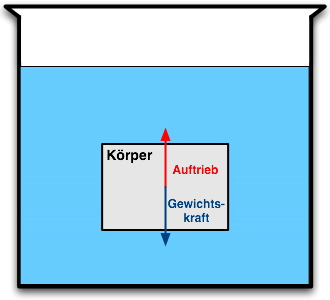
\includegraphics[width=0.75\linewidth]{Bilder/auftrieb} \\
\end{minipage}




	\begin{tabular}{c l c}
		$F_A$ & Auftriebskraft & $[F_A] = \mathrm{N}$ \\
		\rule{0pt}{8pt}$\rho_{Fl}$ & Dichte \textbf{verdrängtes Fluid} & $[\rho_{Fl}] = \mathrm{\frac{kg}{m^3}}$ \\
		$V_K$ & verdrängtes Fluid-Volumen & $[V_K] = \mathrm{m^3}$  \\
		\rule{0pt}{8pt}$g$ & Erdbeschleunigung $g = 9.81 \mathrm{\frac{m}{s^2}}$ & $[g] = \mathrm{\frac{m}{s^2}}$ \\
		$m_{Fl}$ & Masse des \textbf{verdrängten Fluids} & $[m_{Fl}] = \mathrm{kg}$ \\
		$F_{G,Fl}$ & Gewichtskraft \textbf{verdrängtes Fluid} & $[F_{G,Fl}] = \mathrm{N}$ \\
	\end{tabular}
	


\subsection{Oberflächenspannung $\sigma$}

$$ \boxed{ \sigma := \frac{F}{l} } $$ 


	\begin{tabular}{c l c}
		\rule{0pt}{10pt}$\sigma$ & Oberflächenspannung & $[\sigma] = \mathrm{\frac{N}{m}} = \mathrm{\frac{J}{m^2}}$ \\
		$F$ & Kraft & $[F] = \mathrm{N} $ \\
		$l$ & Länge & $[l] = \mathrm{m}$  \\
		\\
	\end{tabular}
	
	\textbf{Die Länge $l$ entspricht der gesamten Berührungslänge  \\
	zwischen Flüssigkeit und Festkörper / Gas} \\
	
	\begin{tabular}{ll}
	Zylinder & $l = 2 \, \pi \, r$ \\
	Lamellen & $l = 2 \, b$  (beidseitig!) \\
	\end{tabular}


\subsection{Grenzflächenspannung}

$$ \boxed{ \sigma_{sl} + \sigma_{lg} \cdot cos \varphi = \sigma_{sg }} $$

\begin{minipage}{0.48\linewidth}
	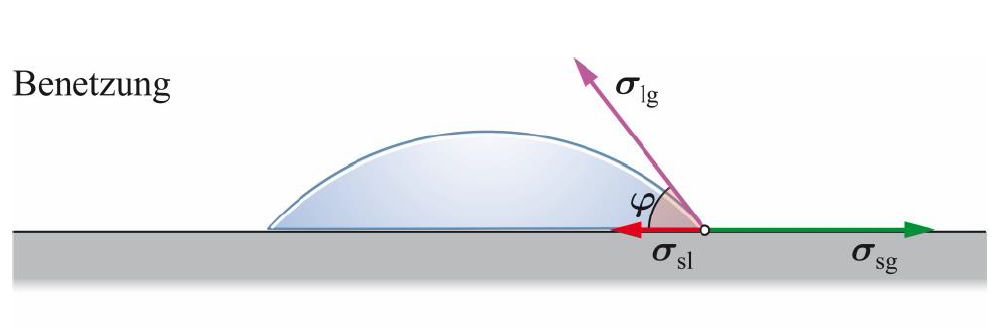
\includegraphics[width=\linewidth]{Bilder/benetzung.png} \\
	$ \varphi < 90 $ %TODO: Winkel einfügen
\end{minipage}
\hfill
\begin{minipage}{0.48\linewidth}
	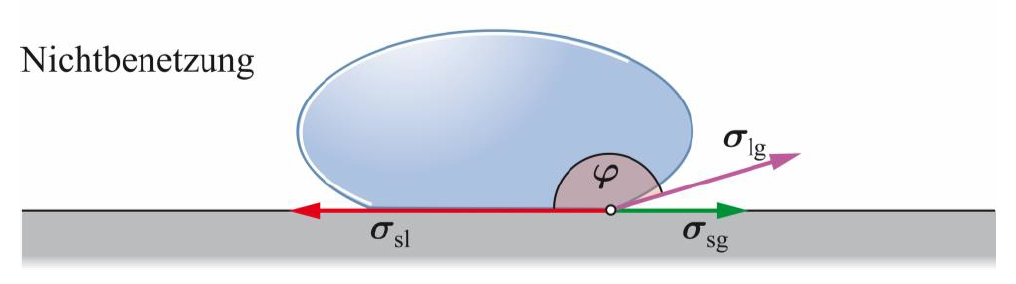
\includegraphics[width=\linewidth]{Bilder/nichtbenetzung.png} \\
	$ \varphi > 90° $
\end{minipage}





\subsection{Kapillarität $h$}

$$\boxed{  h = \frac{2 \cdot \sigma}{\rho \cdot g \cdot r} = \frac{\sigma}{\rho \cdot g \cdot d} }$$ 


	\begin{tabular}{c l c}
		\rule{0pt}{10pt}$\sigma$ & Totale Grenzflächenspannung & $[\sigma] = \mathrm{\frac{N}{m}}$ \\
		\rule{0pt}{10pt}$\rho$ & Dichte der Flüssigkeit & $[\rho] = \mathrm{\frac{kg}{m^3}} $ \\
		\rule{0pt}{10pt}$r$ & Radius der Kapillare & $[r] = \mathrm{m}$  \\
		$d$ & Durchmesser der Kapillare & $[r] = \mathrm{m}$  \\
		\\
	\end{tabular}

\begin{minipage}{0.48\linewidth}
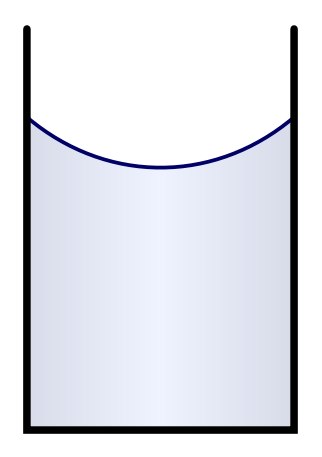
\includegraphics[width=0.3\linewidth]{Bilder/kapillaritaet_benetzend} \\

benetzend
\end{minipage}
\hfill
\begin{minipage}{0.48\linewidth}
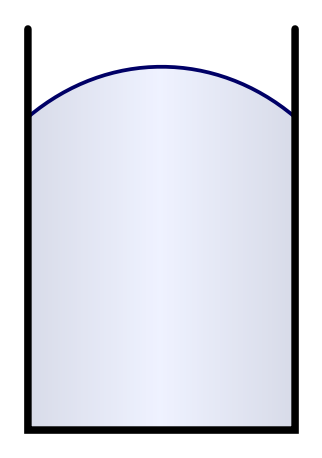
\includegraphics[width=0.3\linewidth]{Bilder/kapillaritaet_nicht_benetzend} \\

nicht benetzend

\end{minipage}




\subsection{Druck in Seifenblase $p$}

$$ \boxed{ p = \frac{2 \cdot \sigma}{r} } $$ 


	\begin{tabular}{c l c}
		\rule{0pt}{8pt}$\sigma$ & Oberflächenspannung & $[\sigma] = \mathrm{\frac{N}{m}}$ \\
		$r$ & Radius der Seifenblase & $[r] = \mathrm{m}$  \\
	\end{tabular}



% \vfill\null
% \columnbreak




\section{Hydrodynamik - Ideale Fluide}

\textbf{Ideale Fluide nehmen keine Scherkräfte auf (keine Reibung) und sind inkompressibel.}

\subsection{Stromlinien-Modell}

\begin{tabular}{ll}
$\bullet$ & Stromlinien zeigen Geschwindigkeit des Fluids \\
$\bullet$ & \textbf{Dichte} Stromlinien bedeutet \textbf{hohe} Geschwindigkeit \\
$\bullet$ & \textbf{Dünne} Stromlinien bedeutet \textbf{niedrige} Geschwindigkeit \\
$\bullet$ & Stationär: Stromlinien = Bahnlinien $\Rightarrow$ schneiden sich nicht 
\end{tabular}




\subsection{Kontinuitätsgleichung}


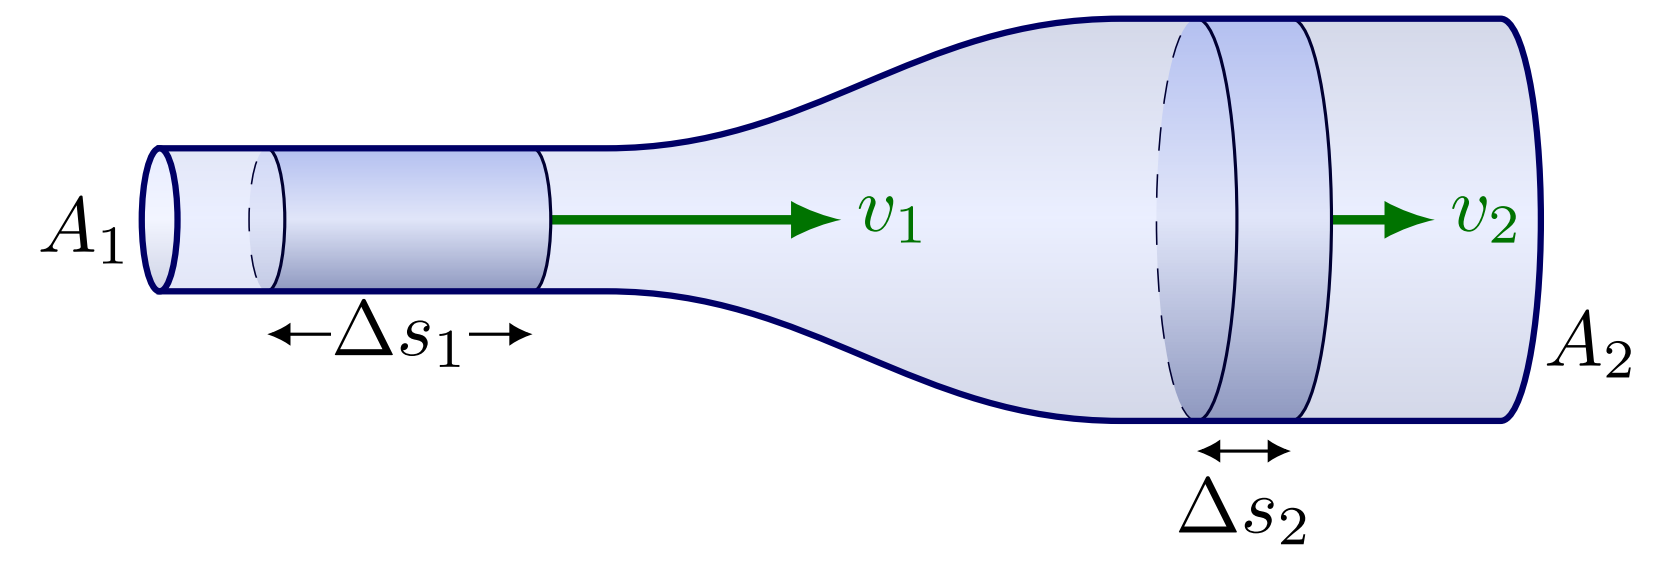
\includegraphics[width=0.7\linewidth]{Bilder/Kontinuitaet.png}


$$ \boxed{ \frac{\Delta V}{\Delta t} = \dot{V} = A \cdot v = \const } \quad \Leftrightarrow \quad \boxed{  A_1 \cdot v_1 = A_2 \cdot v_2 = \frac{\Delta V}{\Delta t} = \dot{V}} $$ 

\begin{tabular}{c l c}
		$\Delta V$ & Volumenänderung & $[\Delta V] = \mathrm{m^3}$ \\
		$\Delta t$ & Zeitänderung & $[\Delta t] = \mathrm{s}$  \\
		\rule{0pt}{8pt}$\dot{V}$ & Volumenstrom (Volumen pro Zeit) & $[\dot{V}] = \mathrm{\frac{m^3}{s}}$ \\
		$A_x$ & Querschnittsfläche & $[A_x] = \mathrm{m^2}$ \\
		\rule{0pt}{8pt}$v_x$ & Geschwindigkeit der Flüssigkeit & $[v_x] = \mathrm{\frac{m}{s}}$ \\
		\\
	\end{tabular}

$\Rightarrow$ Gilt auch für Gase, wenn $v << v_{Schall}$

% \vfill\null
% \columnbreak


\subsection{Bernoulli-Gleichung}

\begin{minipage}{0.38\linewidth}
Die Bernoulli-Gleichung beschreibt ein \\
\underline{bewegtes} Fluid \\
\end{minipage}
\hfill
\begin{minipage}{0.6\linewidth}
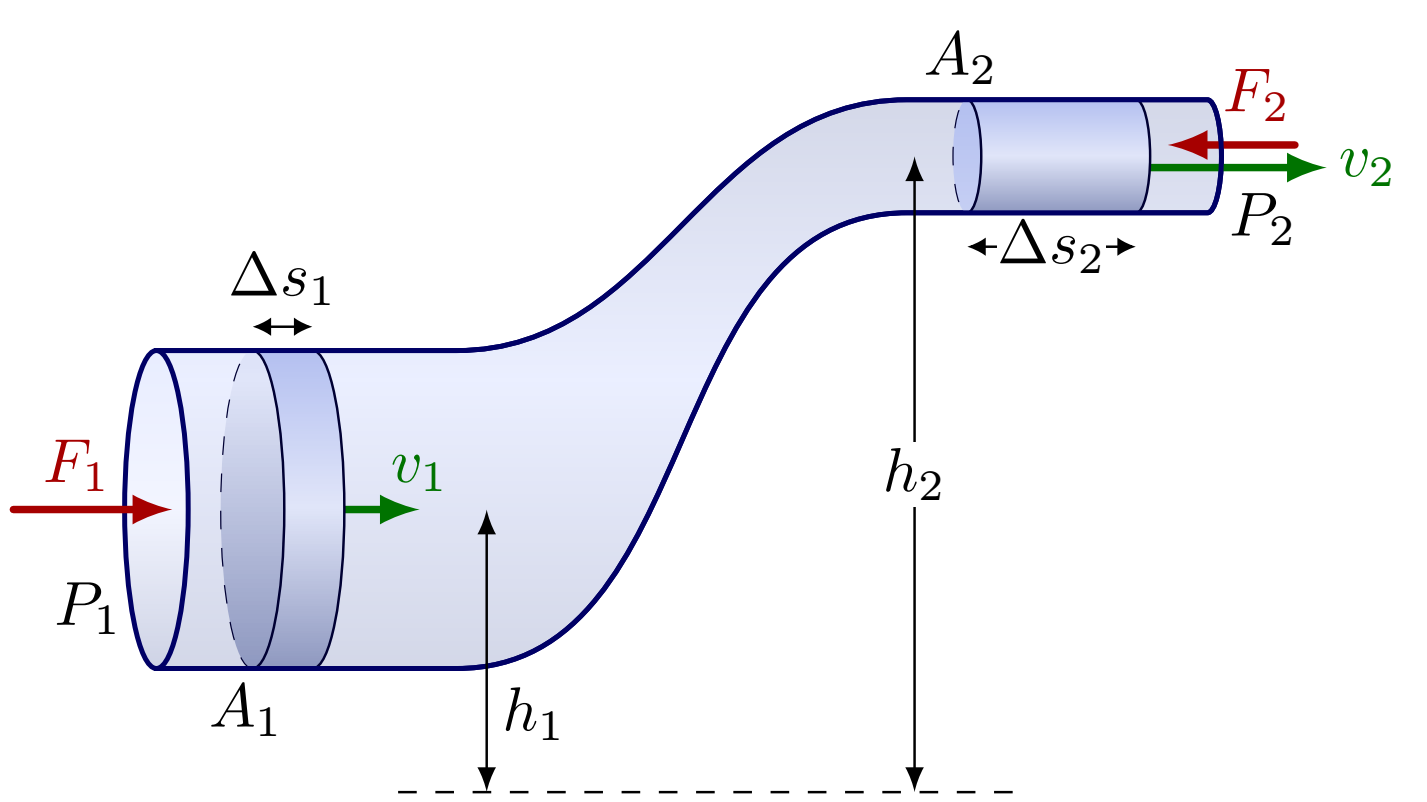
\includegraphics[width=0.99\linewidth]{Bilder/Bernoulli} \\
\end{minipage}








$$ \underbrace{ p + \rho \cdot g \cdot h }_{\substack{\mathrm{statisch}}} + \underbrace{ \frac{1}{2} \, \rho \cdot v^2 }_{\substack{\mathrm{dynamisch}}} = \const $$
	
	$$ \boxed{ p_1 +  \rho \cdot g \cdot h_1 + \frac{1}{2} \, \rho \cdot v_1^2 = p_2 +  \rho \cdot g \cdot h_2 + \frac{1}{2} \, \rho \cdot v_2^2 } $$


\subsubsection{Spezialfall: Horizontal}

$$ \boxed{ p + \frac{1}{2} \, \rho \cdot v^2 = \const } $$


\subsubsection{Spezialfall: Statik}

$$  \boxed{ p + \rho \, \cdot g \cdot h =  \const} $$




\subsubsection{Hydrodynamisches Paradoxon}
\textbf{Je grösser die Strömungsgeschwindigkeit, desto kleiner der Druck} \\


%\vfill\null
%\columnbreak



\subsection{Bernoulli-Gleichung und Energieerhaltung} % eventuell weglassen
Die in der Bernoulli-Gleichung vorkommenden Terme können als \underline{Energie pro Volumen} betrachtet werden \\
\\
\begin{tabular}{l c l}
$  \mathrm{E_{Mech}}$ & $=$ & $\mathrm{elast. \; Energie +  pot. \; Energie + kin. \; Energie}$ \\
\\
& $=$ & $ p \cdot V + m \cdot g \cdot h + \frac{1}{2} \, m \cdot v^2 = \const$ \\
\\
\end{tabular}


Wenn durch das Volumen dividiert wird erhält man: \\
\\
\begin{tabular}{l c l}
$  \mathrm{\frac{E_{Mech}}{Volumen}}$ & $=$ & $\mathrm{\frac{elatische Energie}{Volumen}   + \frac{pot. \; Energie}{Volumen} + \frac{kin. \; Energie}{Volumen}}$ \\
\\
& $=$ & $ p + \rho \cdot g \cdot h + \frac{1}{2} \,  \rho \cdot v^2 =\const$ \\
\\
\end{tabular}


Bei einer horizontalen Strömung entfällt die pot. Energie\\
(pro Volumen) \\
\\

\begin{tabular}{l c l}
$ \mathrm{ \frac{E_{Mech}}{Volumen}}$ & $=$ & $\mathrm{ \frac{elatische Energie}{Volumen} + \frac{kin. \; Energie}{Volumen} }$ \\
\\
& $=$ & $ p + \frac{1}{2} \, \rho \cdot v^2 = \const$ \\
\end{tabular}





\section{Hydrodynamik - Reale Fluide}

\textbf{Reale Fluide nehmen Scherkräfte auf (Reibung)}


\subsection{Newton'sches Reibungs-Gesetz}
Ein \underline{reales Fluid} erfährt \underline{Reibung} 

$$ \boxed{ \tau = \eta \cdot \frac{v}{d} }  \qquad  \boxed{ \tau = \eta \cdot \frac{d \, v}{d \, z} } $$

\begin{tabular}{c l c}
		$\tau$ & Schubspannung & $[\tau] = \mathrm{N}$ \\
		$\eta$ & dynmaische Zähigkeit (Viskosität) & $[\eta] = \mathrm{Pa \cdot s}$ \\
		\rule{0pt}{8pt}$v$ & Geschwindigkeitsdifferenz zw. Auflagen & $[v] = \frac{m}{s}$ \\
		$z$ & Richtung senkrecht zur Verschiebung & $[z] = \mathrm{m}$ \\
		$d$ & Distand zwischen den Auflagen & $[d] = \mathrm{m}$ \\
		\rule{0pt}{8pt}$\frac{d \, v}{d \, z}$ & Geschwindigkeits-Gradient in z-Richtung & $[\frac{d \, v}{d \, z}] = \mathrm{\frac{1}{s}}$ \\
		\\
\end{tabular}
	
\textbf{Beispiele: Werte für $\eta$} \\ %TODO: Gradzeichen fixen!
\\
\begin{tabular}{l c l}
		$\eta_{Luft}$ & $:=$ & $17 \cdot 10^{-6} \; \mathrm{Pa \cdot s} $ \\
		$\eta_{Wasser} (20°C)$ & $:=$ & $10^{-2} \; \mathrm{Pa \cdot s}$ \\
		$\eta_{Oel}$ & $:=$ & $0.1 \; \mathrm{Pa \cdot s}$ bis $1 \; \mathrm{Pa \cdot s}$ \\
\end{tabular}


\subsubsection{Kinematische Zähigkeit $\nu$}

$$ \boxed{ \nu = \frac{\eta}{\rho}  } $$

\begin{tabular}{c l c}
		\rule{0pt}{8pt}$\nu$ & kinematische Zähigkeit & $[\nu] = \mathrm{\frac{m^2}{s}}$ \\
		\rule{0pt}{8pt}$\rho$ & Dichte & $[\rho] = \mathrm{\frac{kg}{m^3}}$  \\	
\end{tabular}
	

	
\subsection{Stokes'sche Reibung $F_R$}
Z.B. für Kugel in Öl oder fallende Wassertropfen

$$ \boxed{ F_R = 6 \cdot \pi \cdot \eta \cdot R \cdot v } $$

\begin{tabular}{c l c}
		$F_R$ & Reibungskraft & $[F_R] = \mathrm{N}$ \\
		$\eta$ & Dynamische Zähigkeit (Viskosität) & $[\eta] = \mathrm{Pa \cdot s}$  \\
		$R$ & Kugelradius & $[R] = \mathrm{m}$ \\
		\rule{0pt}{8pt}$v$ & Geschwindigkeit & $[v] = \mathrm{\frac{m}{s}}$		
\end{tabular}


\subsubsection{Kugelfall-Viskosimeter}
Auf eine Kugel, welche in einer Flüssigkeit hinabgleitet wirken \\
folgende Kräfte: \\
\\
\begin{minipage}{0.4\linewidth}
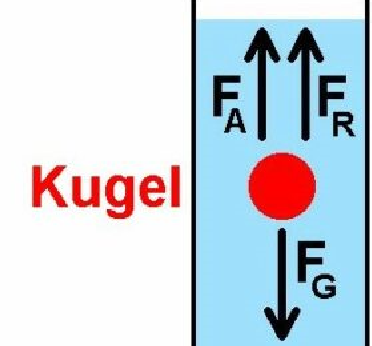
\includegraphics[width=0.8\linewidth]{Bilder/kugelfall-viskosimeter} \\
\end{minipage}
\hfill
\begin{minipage}{0.53\linewidth}
\begin{tabular}{ll}
$F_G$ & Gewichtskraft \\
$F_A$ & statischer Auftrieb \\
$F_R$ & Stokes'sche Reibung \\
\\
\end{tabular}

Ansatz zum Lösen von Aufgaben: \textbf{Kräftegleichgewicht}
\end{minipage}






% \vfill\null
% \columnbreak


\subsection{Hagen-Poiseuille}
Beschreibung von \underline{laminaren} Strömungen in einem \underline{runden Rohr} \\
$\Rightarrow$ Schichtströmung

\subsubsection{Gesetz von Hagen-Poiseuille}

$$ \boxed{ \dot{V} = \frac{\pi \cdot \Delta \, p \cdot R^4}{8 \cdot \eta \cdot l} } $$
 
\subsubsection{Geschwindigkeitsverteilung von $r=0$ bis R}

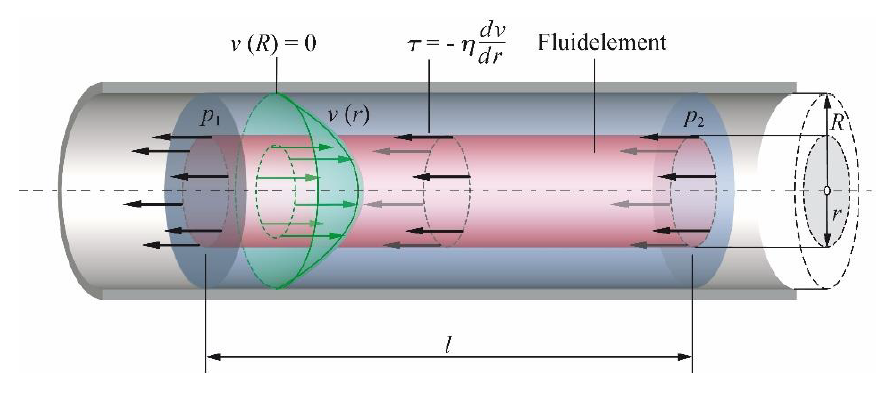
\includegraphics[width=0.8\linewidth]{Bilder/laminare_geschwindigkeit.png}

$$ \boxed{ v(r) = \frac{1}{4 \cdot \eta} \cdot \frac{\Delta \, p}{l} \, (R^2 - r^2) } $$



\begin{tabular}{c l c}
		\rule{0pt}{8pt}$v(r)$ & Fliessgeschwindigkeit beim Radius $r$ & $[v(r)] = \mathrm{\frac{m}{s}}$ \\
		$r$ & betrachteter Radius & $[r] = \mathrm{m}$ \\
		$\eta$ & Dynamische Zähigkeit (Viskosität) & $[\eta] = \mathrm{Pa \cdot s}$  \\
		$R$ & Rohr-(Innen)Radius & $[R] = \mathrm{m}$ \\
		$\Delta \, p$ & Druckdifferenz & $[\Delta \, p] = \mathrm{Pa}$ \\
		\rule{0pt}{8pt}$\dot{V} = \frac{d \, V}{d \, t}$ &  Volumenstrom & $[\dot{V}] = \mathrm{\frac{m^3}{s}}$	 \\
		$l$ & Länge des Rohrs & $[l] = \mathrm{m}$
\end{tabular}



\subsection{Reynolds-Zahl $Re$}
Gibt ein Richtmass für die Wirbelbildung  \\
\\
$\bullet$ Druck-Differenz (Bernoulli) begünstigt Wirbelbildung \\
$\bullet$ Innere Reibung (Schubspannung) verhindert Wirbelbildung 

$$\boxed{  Re = \frac{\Delta \, p}{\tau} = \frac{\rho \cdot \overline{v} \cdot d}{\eta} \qquad \qquad \mathrm{mit} \; \; \overline{v} = \frac{\dot{V}}{A} }  $$

	
\begin{tabular}{c l c}
		$Re$ & Reynolds-Zahl & $[Re] = 1$ \\
		$\eta$ & Dynamische Zähigkeit (Viskosität) & $[\eta] = \mathrm{Pa \cdot s}$  \\
		$\overline{v}$ & Mittlere Geschwindigkeit & $[\overline{v}] = \mathrm{\frac{m}{s}}$ \\
		$d$ & Typische Dimension (Rohrdurchmesser) & $[d] = \mathrm{m}$ \\
		$\Delta \, p$ & Druckdifferenz & $[\Delta p] = \mathrm{Pa}$ \\
		$\tau$ & Schubspannung & $[\tau] = \mathrm{N}$ \\
		\\
\end{tabular}

\textbf{Sobald die Reynolds-Zahl $Re$ grösser ist als ein kritischer Wert bilden sich Wirbel} \\
\\
$\Rightarrow$ Rohr:  $Re_{kritisch} \approx 2320$


\subsubsection{Ähnlichkeitsgesetz}
Reynolds-Zahl dient auch richtigem Vergleich von Modellversuchen. \\
\\
$\Rightarrow$ Gleiche Reynolds-Zahl bedeutet gleiches Verhalten \\
\\
$\Rightarrow$ Gleiche Reynolds-Zahl bedeutet auch gleiche \\
 Relative Grenzschicht-Dicke $D$ (siehe \ref{Grenzschichtdicke})



\vfill\null
\columnbreak


\subsection{Turbulente / Laminare Rohrströmung}

\subsubsection{Hilfe, um Reynoldszahl zu bestimmen (laminar)}

$$ \boxed{ \Delta p = 32 \cdot \eta \cdot l \cdot \frac{v}{d^2} }  $$


\subsubsection{Druckunterschied in laminare / turbulente Strömung}

$$ \lambda_{turbulent} = \frac{0.316}{\sqrt[4]{Re}}  \qquad \qquad \lambda_{laminar} = \frac{64}{Re}  $$

$$ \boxed{ \Rightarrow \Delta p_x = \lambda_x \frac{l}{d} \cdot \frac{\rho}{2} \cdot v^2 } $$



\begin{tabular}{c l c}
		$\Delta \, p_x$ & Druckdifferenz (laminar/turbulent) & $[\Delta p] = \mathrm{Pa}$ \\
		$\eta$ & Dynamische Zähigkeit (Viskosität) & $[\eta] = \mathrm{Pa \cdot s}$  \\
		$l$ & Rohr-Länge & $[l] = \mathrm{m}$ \\
		\rule{0pt}{8pt}$v$ & Fliess-Geschwindigkeit & $[v] = \mathrm{\frac{m}{s}}$ \\
		$d$ & Rohr-Durchmesser & $[d] = \mathrm{m}$ \\		
		\rule{0pt}{8pt}$\rho$ & Dichte des Fluids & $[\rho] = \mathrm{\frac{kg}{m^3}}$ \\
		$Re$ & Reynolds-Zahl & $[Re] = 1$ \\
\end{tabular}




\subsubsection{Unbekannt / Gemischt (Pratische Anwendung)}
Vorgehen, wenn man nicht weiss, ob sich Wirbel bilden oder nicht \\
\\
\begin{tabular}{ll}
1. & Laminar rechnen (um fehlenden Parameter $\rho, \; v, \; d, \; \mathrm{oder} \; \eta$ \\
   &  zu bestimmen) \\
2. & Aus Resultat Reynolds-Zahl berechnen \\
3. & Mit kritischer Reynolds-Zahl vergleichen \\
4. & Beim \textbf{Überschreiten} $\Rightarrow$ Turbulent rechnen! \\
\end{tabular}



\subsection{Prandl'sche Grenzschicht-Dicke $D$}\label{Grenzschichtdicke}
Prandl'sche Grenzschicht-Dicke $D$ beschreibt, in welcher \textbf{Distanz} die \textbf{Geschwindigkeit} eines laminar bewegten Teils (z.B. ein \\
Flugzeugflügel) \textbf{Null} ist. 

$$\boxed{ D = \sqrt{\frac{\eta}{\rho} \cdot \frac{l}{v}} }$$


\begin{tabular}{c l c}
		$D$ & Prandl'sche Grenzschicht-Dicke & $[D] = \mathrm{m}$ \\
		$\eta$ & Dynamische Zähigkeit (Viskosität) & $[\eta] = \mathrm{Pa \cdot s}$  \\
		\rule{0pt}{8pt}$\rho$ & Dichte des Fluids & $[\rho] = \mathrm{\frac{kg}{m^3}}$ \\
		$l$ & Länge des bewegten Teils (in Richtung von $v$) & $[l] = \mathrm{m}$ \\
		\rule{0pt}{8pt}$v$ & Geschwindigkeit & $[v] = \mathrm{\frac{m}{s}}$ \\
			\\
\end{tabular}

\begin{minipage}{0.48\linewidth}
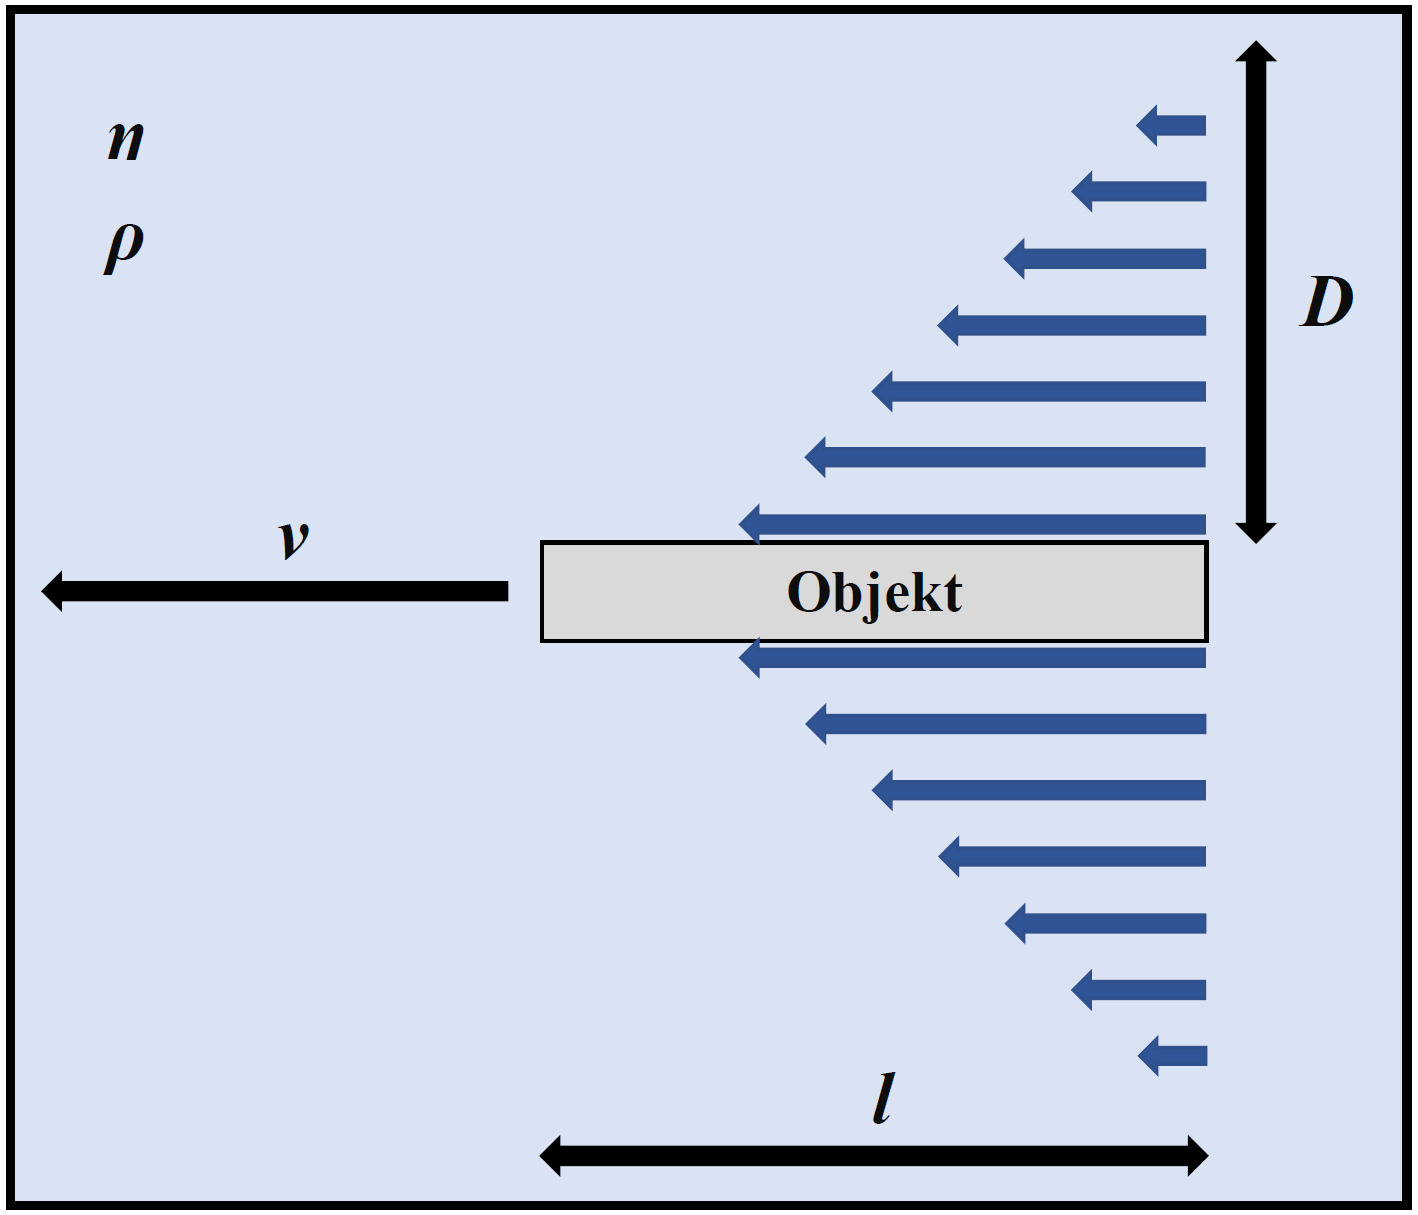
\includegraphics[width=0.8\linewidth]{Bilder/prandl}
\end{minipage}
\hfill
\begin{minipage}{0.48\linewidth}
Die Geschwindigkeit innerhalb der Grenzschicht $D$ nimmt vom Teil bis hin zum äussersten Rand \textbf{linear} ab.
\end{minipage}


% \vfill\null
% \columnbreak




\subsection{Bernoulli-Gleichung mit innerer Reibung}

$$ \boxed{  p_1 +  \rho \cdot g \cdot h_1 + \frac{1}{2} \, \textcolor{red}{\alpha_1} \cdot \rho \cdot v_1^2 = p_2 +  \rho \cdot g \cdot h_2 + \frac{1}{2} \, \textcolor{red}{\alpha_2} \cdot \rho \cdot v_2^2 \textcolor{red}{+ \Delta \, p_v}  }$$

\begin{tabular}{c| c |c}
 & turbulent & laminar \\ 
\hline 
Korrekturfaktoren & $\alpha_1 \approx \alpha_2 \approx 2$  & $\alpha_1 \approx \alpha_2 \approx 1$ \\ 
\hline 
\rule{0pt}{11pt} Druckverlust $\Delta \, p_v$ & \multicolumn{2}{c}{$\Delta p_v = \lambda_x \frac{l}{d} \cdot \frac{\rho}{2} \cdot v^2$} \\ 
\hline 
\rule{0pt}{11pt}  & $\lambda_{turbulent} = \frac{0.316}{\sqrt[4]{Re}}  $ & $\lambda_{laminar} = \frac{64}{Re} $  \\ 
\end{tabular} 



\subsection{Druckwiderstand $F_D$}
Bezeichnet die turbulente Luftreibungskraft $F_R$ und wird meist als Luftwiderstand bezeichnet \\

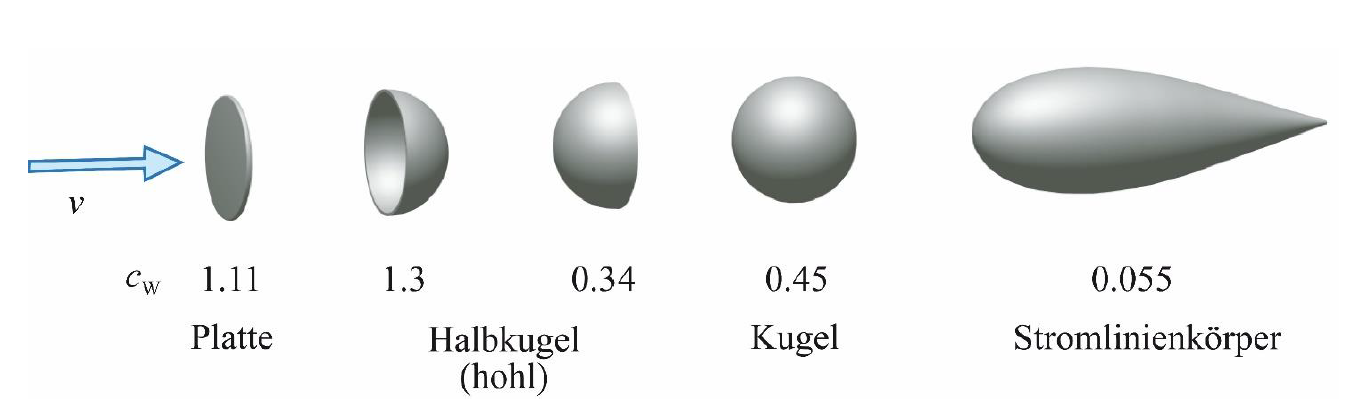
\includegraphics[width=0.8\linewidth]{Bilder/widerstandsbeiwert.png}

$$ \boxed{ F_D = \Delta \, p \cdot A_s = \frac{1}{2} \, \cdot \rho \cdot v^2 \cdot A_s \cdot c_W } $$


\begin{tabular}{c l c}
		$F_D$ & Druckwiderstand & $[F_D] = \mathrm{N}$ \\
		$\Delta \, p$ & Druckdifferenz & $[\Delta \, p] = \mathrm{Pa}$  \\
		\rule{0pt}{8pt}$\rho$ & Luft-Dichte & $[\rho] = \mathrm{\frac{kg}{m^3}}$ \\
		\rule{0pt}{8pt}$v$ & Strömungs-Geschwindigkeit & $[v] = \mathrm{\frac{m}{s}}$ \\
		$c_W$ & Widerstandsbeiwert / Widerstandszahl & $[c_W] = 1$\\
		$A_s$ & projizierte Fläche senkrecht zur Strömung & $[A_s] = \mathrm{m^2}$ \\
		\\
\end{tabular}

Der Widerstandsbeiwert $c_W$ ist \textbf{geometrieabhängig}!






\subsection{Auftriebskraft $F_A$ nach Kutta-Jukowski}
Beschreibt Proportionalität zwischen dynamischem Auftrieb \\
und Zirkulation 

$$ \boxed{ F_A = \rho \cdot v \cdot l \cdot \Gamma } $$

\begin{tabular}{c l c}
		$F_A$ & dynamischer Auftrieb & $[F_A] = \mathrm{N}$ \\
		\rule{0pt}{8pt}$\rho$ & Dichte des Fluids & $[\rho] = \mathrm{\frac{kg}{m^3}}$ \\
		\rule{0pt}{8pt}$v$ & Geschwindigkeit & $[v] = \mathrm{\frac{m}{s}}$ \\
		$l$ & Länge quer zur Strömung & $[l] = \mathrm{m}$ \\
		\rule{0pt}{8pt}$\Gamma$ & Zirkulation & $[\Gamma] = \mathrm{\frac{m^2}{s}}$ \\
\end{tabular}






\subsubsection{Zirkulation $\Gamma$}
Die Zirkulation ist ein Mass für die \textbf{Rotation} im Strömungsfeld \\

$$ \boxed{ \Gamma = 	\oint \vec{v} \bullet d\vec{s} } $$


\begin{tabular}{c l c}
		\rule{0pt}{8pt}$\Gamma$ & Zirkulation & $[\Gamma] = \mathrm{\frac{m^2}{s}}$ \\
		\rule{0pt}{8pt}$\vec{v} \bullet d\vec{s}$ & Geschwindigkeit entlang dem Weg & $[\vec{v}] = \mathrm{\frac{m}{s}}$  \\
		& (Skalarprodukt: $\vec{v} \bullet d\vec{s} = a \cdot b \cdot \cos(\varphi)$ & \\
\end{tabular} \\
\\
\textbf{Rotierender Zylinder:} $$ \boxed{ \Gamma = 2\pi r v_{Zyl} = 4\pi^2r^2f } $$


% \vfill\null
% \columnbreak



\subsection{Dynamischer Auftrieb $F_A$}

$$ \boxed{ F_A = c_A \cdot  \underbrace{\frac{1}{2} \cdot \rho \cdot v^2 }_{\substack{\Delta \, p}} \cdot A_{\|}	} $$


\begin{tabular}{c l c}
		$F_A$ & dynamischer Auftrieb & $[F_A] = \mathrm{N}$ \\
		$c_A$ & Auftriebskoeffizient & $[c_A] = 1$ \\
		\rule{0pt}{8pt}$\rho$ & Luft-Dichte & $[\rho] = \mathrm{\frac{kg}{m^3}}$ \\
		\rule{0pt}{8pt}$v$ & Strömungsgeschwindigkeit & $[v] = \mathrm{\frac{m}{s}}$ \\
		$A_{\|}$ & Projizierte Fläche \textbf{parallel} zur Strömung & $[A_{\|}] = \mathrm{m^2}$ \\
\end{tabular}




\subsubsection{Wissenswertes zum dynamischen Auftrieb}
Ein gerade ausgerichtetes, symmetrisches Stromlinienprofil erzeugt \textbf{keinen} dynamischen Auftrieb \\
\\
An einem asymmetrischen Flügelprofil entsteht dynamischer\\
Auftrieb 


\subsection{Induzierter Widerstand $F_W$}
Kommt durch Energieverlust (Wirbelbildung) zu Stande, welcher entsteht, wenn die Umgebungsluft in Bewegung gesetzt wird

$$ \boxed{ F_W = c^*_W \cdot \frac{1}{2} \cdot \rho \cdot v^2 \cdot A_{\|} } $$


\begin{tabular}{c l c}
		$F_W$ & Induzierter Widerstand & $[F_W] = \mathrm{N}$ \\
		$c^*_W$ & Widerstands-Koeffizient & $[c*_W] = 1$ \\
		\rule{0pt}{8pt}$\rho$ & Luft-Dichte & $[\rho] = \mathrm{\frac{kg}{m^3}}$ \\
		\rule{0pt}{8pt}$v$ & Strömungsgeschwindigkeit & $[v] = \mathrm{\frac{m}{s}}$ \\
		$A_{\|}$ & Projizierte Fläche \textbf{parallel} zur Strömung & $[A_{\|}] = \mathrm{m^2}$ \\
\end{tabular}


\subsection{Gleitwinkel $\varphi$}
Gibt die zurückgelegte Stecke pro verbrauchte Höhe an \\
Im Luft-Kanal ist dies der Anstell-Winkel \\

\begin{minipage}{0.5\linewidth}
	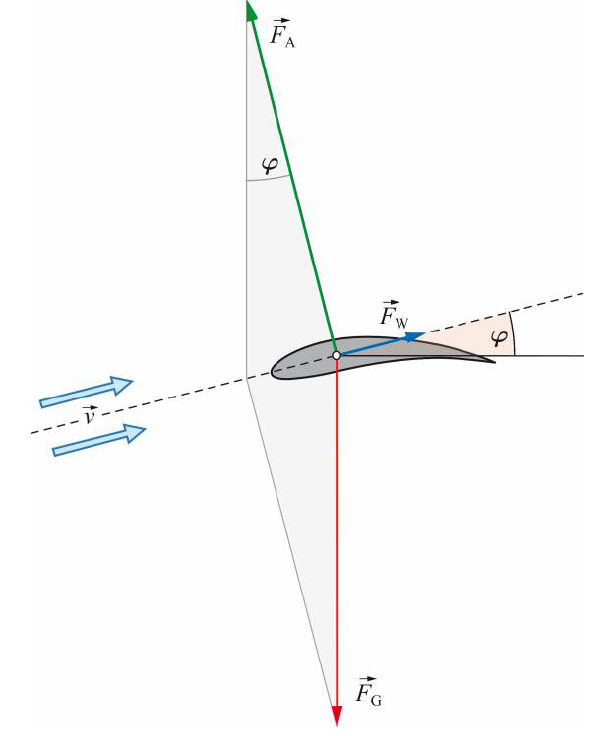
\includegraphics[width=\linewidth]{Bilder/gleitwinkel.png}
\end{minipage}
\hfill
\begin{minipage}{0.45\linewidth}
	$$ \boxed{ tan(\varphi) = \frac{F_W}{F_A} = \frac{c^*_W}{c_A}= \frac{v_V}{v_H} }	$$
\end{minipage}






\begin{tabular}{c l c}
		$\varphi$ & Gleitwinkel & $[\varphi] = \text{°}$ \\
		$F_W$ & Widerstandskraft & $[F_W] = \mathrm{N}$ \\
		$F_A$ & Auftriebskraft & $[F_A] = \mathrm{N}$ \\ 
		$c^*_W$ & Widerstands-Koeffizient & $[c^*_W] = 1$ \\
		$c_A$ & Auftriebs-Koeffizient & $[c_A] = 1$ \\
		\rule{0pt}{8pt}$v_V$ & Vertikal-Geschwindigkeit & $[v_V] = \mathrm{\frac{m}{s}}$ \\
		\rule{0pt}{8pt}$v_H$ & Horizontal-Geschwindigkeit & $[v_H] = \mathrm{\frac{m}{s}}$ \\
\end{tabular}

\subsubsection{Gängige Gleitzahlen}
\begin{center}
    \begin{tabular}{lc}
        \textbf{Flugobjekt} & \textbf{Gleitzahl}\\ \hline
		Hängegleiter  & 10 bis 15 \\
		Boeing 747    & 15 \\
		Airbus A380   & 20 \\
		Segelflugzeug &	40 (Rekord 70) \\
	\end{tabular}
\end{center}


\subsection{Helmholz'sche Wirbelsätze}
\begin{tabular}{ll}
1. & Wirbel hat kein Anfang und kein Ende \\
2. & Wirbel besteht immer aus denselben Fluidteilchen \\
3. & Zirkulation zeitlich konstant \\
\end{tabular}

% \vfill\null
% \columnbreak